\documentclass{article}

\usepackage{graphicx}
\usepackage{tikz}
\usepackage{tikzsymbols}
\usetikzlibrary{calc,patterns,shapes.geometric}
\pagestyle{empty}
\usepackage[margin=0pt]{geometry}
\geometry{papersize={14in,12in}}

\def\centerarc[#1](#2)(#3:#4:#5){\draw[#1] ($(#2)+({#5*cos(#3)},{#5*sin(#3)})$) arc (#3:#4:#5);}

\begin{document}
	\begin{figure}
		\centering
		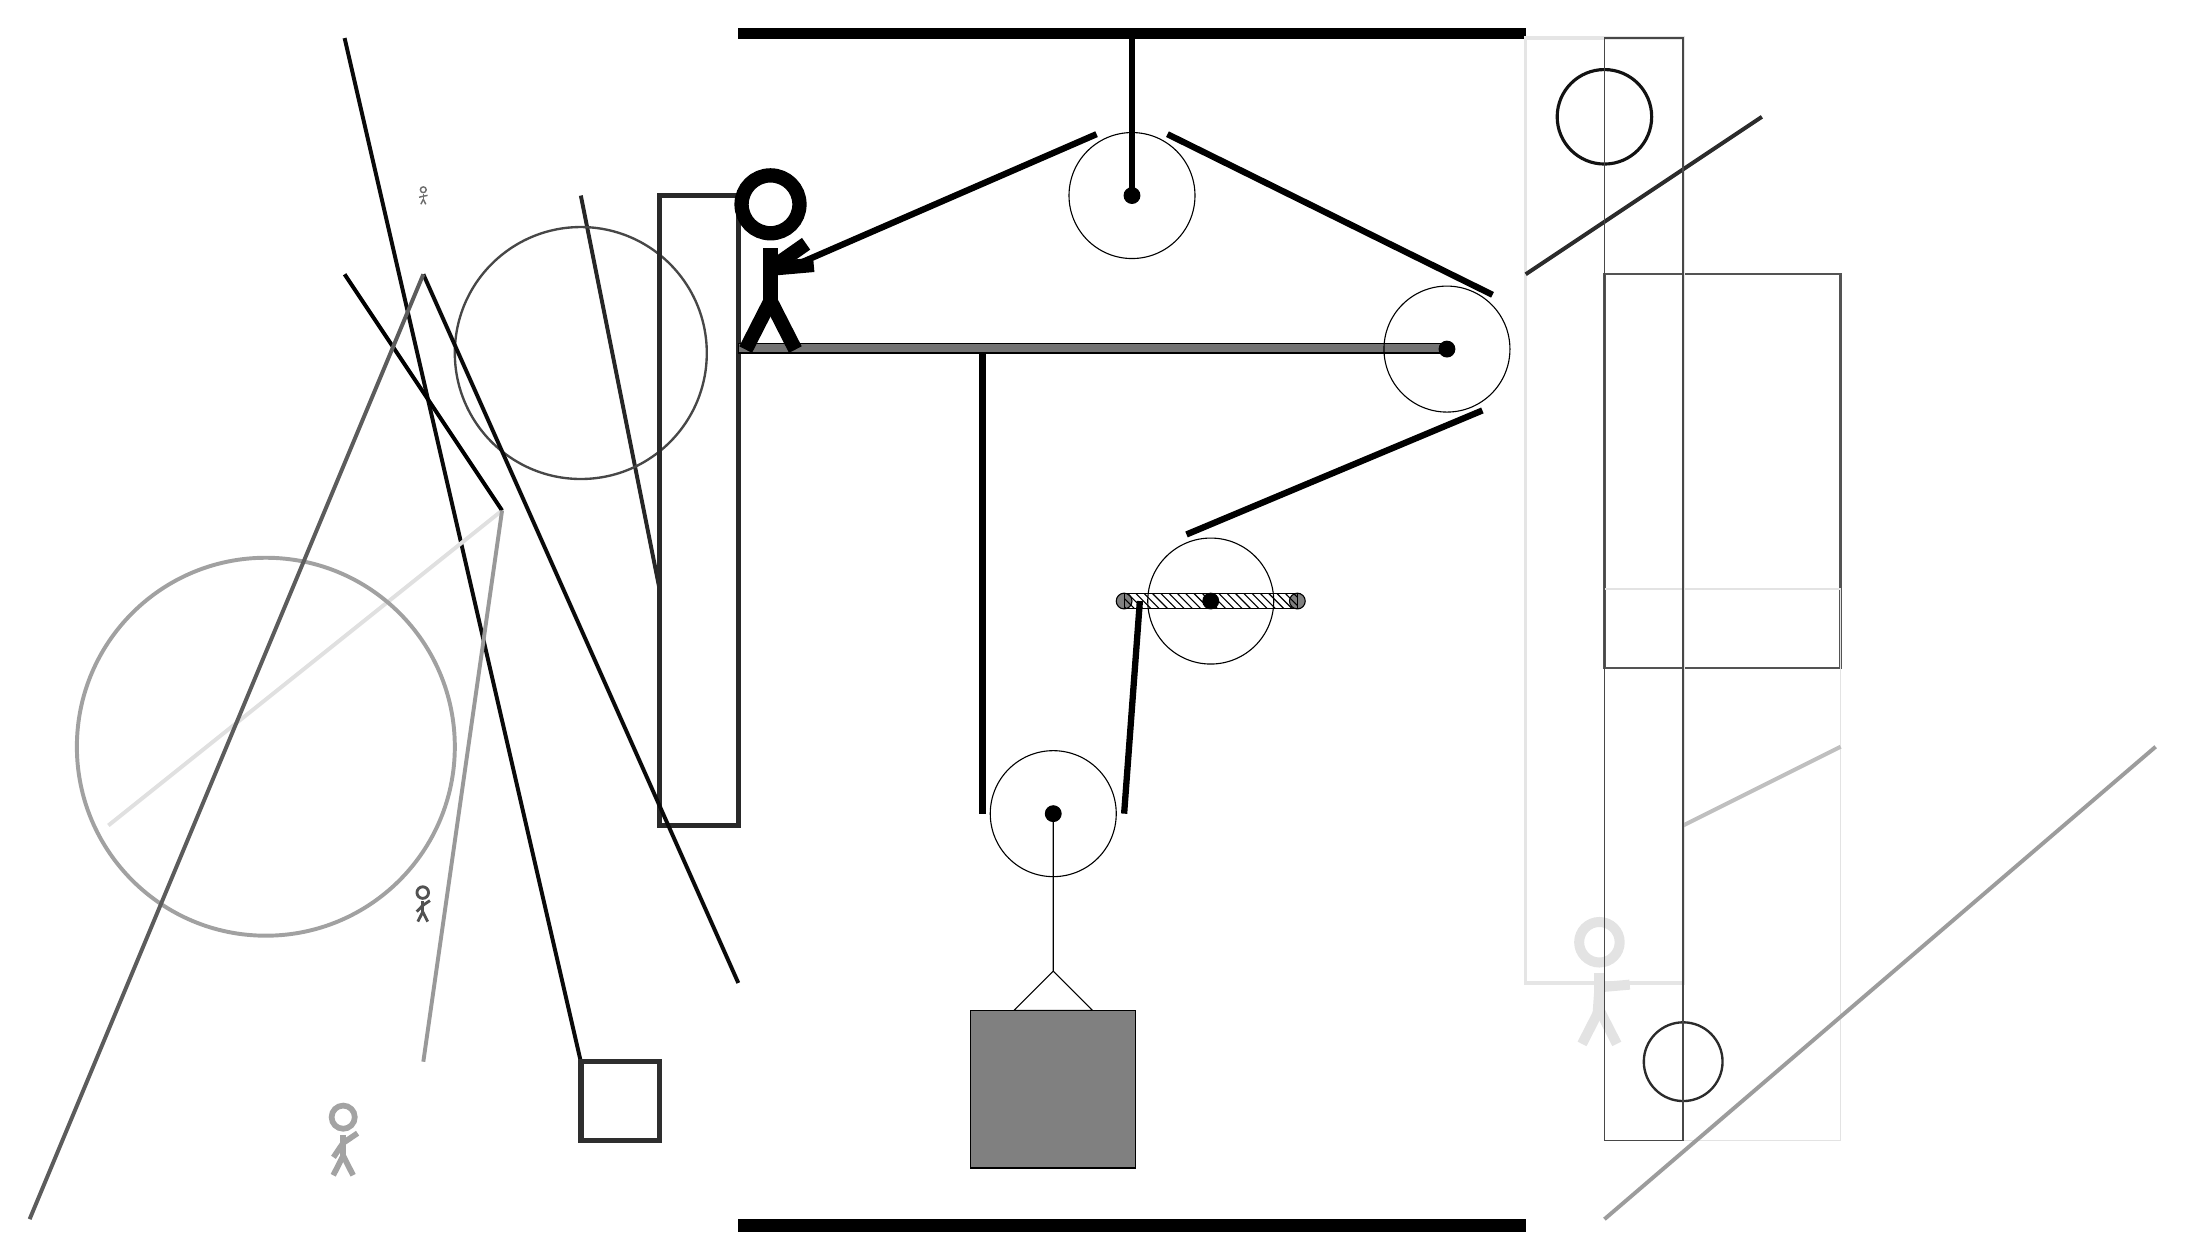
\begin{tikzpicture}
			%%%%% START %%%%%
			
			\draw[fill=black] (-2, 13) rectangle (8, 13.125);
			
			\draw[line width=0.3mm, color=black!67] (9, 10) rectangle (12, 5);
			
			\draw[line width=0.2mm, color=black!11] (9, -1) rectangle (12, 6);
			\draw[line width=0.5mm, color=black!85](-4, 11) -- (-3, 6);
			\draw[line width=0.5mm, color=black!96](-7, 13) -- (-4, 0);
			\draw [line width=0.3mm, color=black!83](10, 0) circle (0.5);
			
			\draw[line width=0.5mm, color=black!39](9, -2) -- (16, 4);
			\draw[line width=0.4mm, color=black!10] (8, 13) rectangle (10, 1);
			\node[line width=0.5mm, color=black!57] at (-6, 11) {\Strichmaxerl[1][15][10]};
			\node[line width=0.4mm, color=black!68] at (-6, 2) {\Strichmaxerl[2][46][34]};
			
			\draw [line width=0.3mm, color=black!72](-4, 9) circle (1.6);
			\draw[line width=0.5mm, color=black!12](-5, 7) -- (-10, 3);
			\draw[line width=0.5mm, color=black!100](-5, 7) -- (-7, 10);
			\draw[line width=0.6mm, color=black!84] (-2, 11) rectangle (-3, 3);
			
			\draw [line width=0.4mm, color=black!93](9, 12) circle (0.6);
			\draw[line width=0.5mm, color=black!40](-5, 7) -- (-6, 0);
			\draw [line width=0.5mm, color=black!37](-8, 4) circle (2.4);
			
			\node[line width=0.7mm, color=black!11] at (9, 1) {\Strichmaxerl[7][86][5]};
			\draw[line width=0.7mm, color=black!82] (-4, 0) rectangle (-3, -1);
			\draw[line width=0.5mm, color=black!96](-2, 1) -- (-6, 10);
			\draw[line width=0.5mm, color=black!64](-6, 10) -- (-11, -2);
			\draw[line width=0.5mm, color=black!83](8, 10) -- (11, 12);
			\draw[line width=0.5mm, color=black!25](12, 4) -- (10, 3);
			
			\node[line width=0.7mm, color=black!36] at (-7, -1) {\Strichmaxerl[4][56][34]};
			\draw[line width=0.2mm, color=black!72] (9, 13) rectangle (10, -1);
			
			\draw[fill=black!55] (-2, 9) rectangle (7, 9.125);
			
			\draw (2, 3.15) circle (0.8);
			\draw[fill=black] (2, 3.15) circle (0.1);
			
			\draw (7, 9.05) circle (0.8);
			\draw[fill=black] (7, 9.05) circle (0.1);
			
			\draw[fill=white](4, 5.85) circle (0.8);
			\draw[fill=black] (4, 5.85) circle (0.1);
			\draw[fill=black!50] (2.9, 5.85) circle (0.1);
			\draw[fill=black!50] (5.1, 5.85) circle (0.1);
			\draw[pattern=north west lines, pattern color=black] (2.9, 5.95) rectangle (5.1, 5.75);
			
			\draw (3, 11) circle (0.8);
			\draw[fill=black] (3, 11) circle (0.1);
			\draw[line width=0.8mm] (3, 11) -- (3, 13);
			
			\draw (2, 3.15) -- (2, 1.15) -- (1.5, 0.65) -- (2.5, 0.65) -- (2, 1.15);
			\draw[fill=black!50] (0.95, 0.65) rectangle (3.05, -1.35);
			
			\draw[line width=0.8mm] (1.1, 9) -- (1.1, 3.15);
			\centerarc[line width=0.8mm](2, 3.15)(180:360:0.9);
			\draw[line width=0.8mm](2.9, 3.15) -- (3.1, 5.85);
			\centerarc[line width=0.8mm](4, 5.85)(110:180:0.9);
			\draw[line width=0.8mm](3.6922, 6.6957) -- (7.45, 8.2706);
			\centerarc[line width=0.8mm](7, 9.05)(-60:50:0.9);
			\draw[line width=0.8mm](7.5785, 9.7394) -- (3.45, 11.7794);
			\centerarc[line width=0.8mm](3, 11)(60:120:0.9);
			\draw[line width=0.8mm](2.55, 11.7794) -- (-1.2, 10.15);
			
			\node at (-1.5, 10.15) {\Strichmaxerl[10][-175][35]};
			
			\draw[fill=black] (-2, -2) rectangle (8, -2.15);
			
			%%%%% END %%%%%
		\end{tikzpicture}
	\end{figure}	
\end{document}